\section{Case}
\label{sec:hardware:case}

The power supplies for all electronic components are placed in a box together with the Ultra96-V2.
The box is a case from Fibox with a transparent lid to give visitors an impression of how it works.
It features a \SI{230}{VAC} power cable, a \SI{24}{VDC} output for the lighting, a \acrlong{mdp} cable for the monitor and the USB cable for the camera.
In addition, there are three fans on the walls, which provide cooling for the Ultra96-V2 and the power supplies.
The box also contains terminal blocks and cable ducts to store cables that are too long.
All components are mounted on a metal plate.
Figure \ref{fig:fibox3d} shows a 3D model of the box.

\begin{figure}[h]
  \centering
  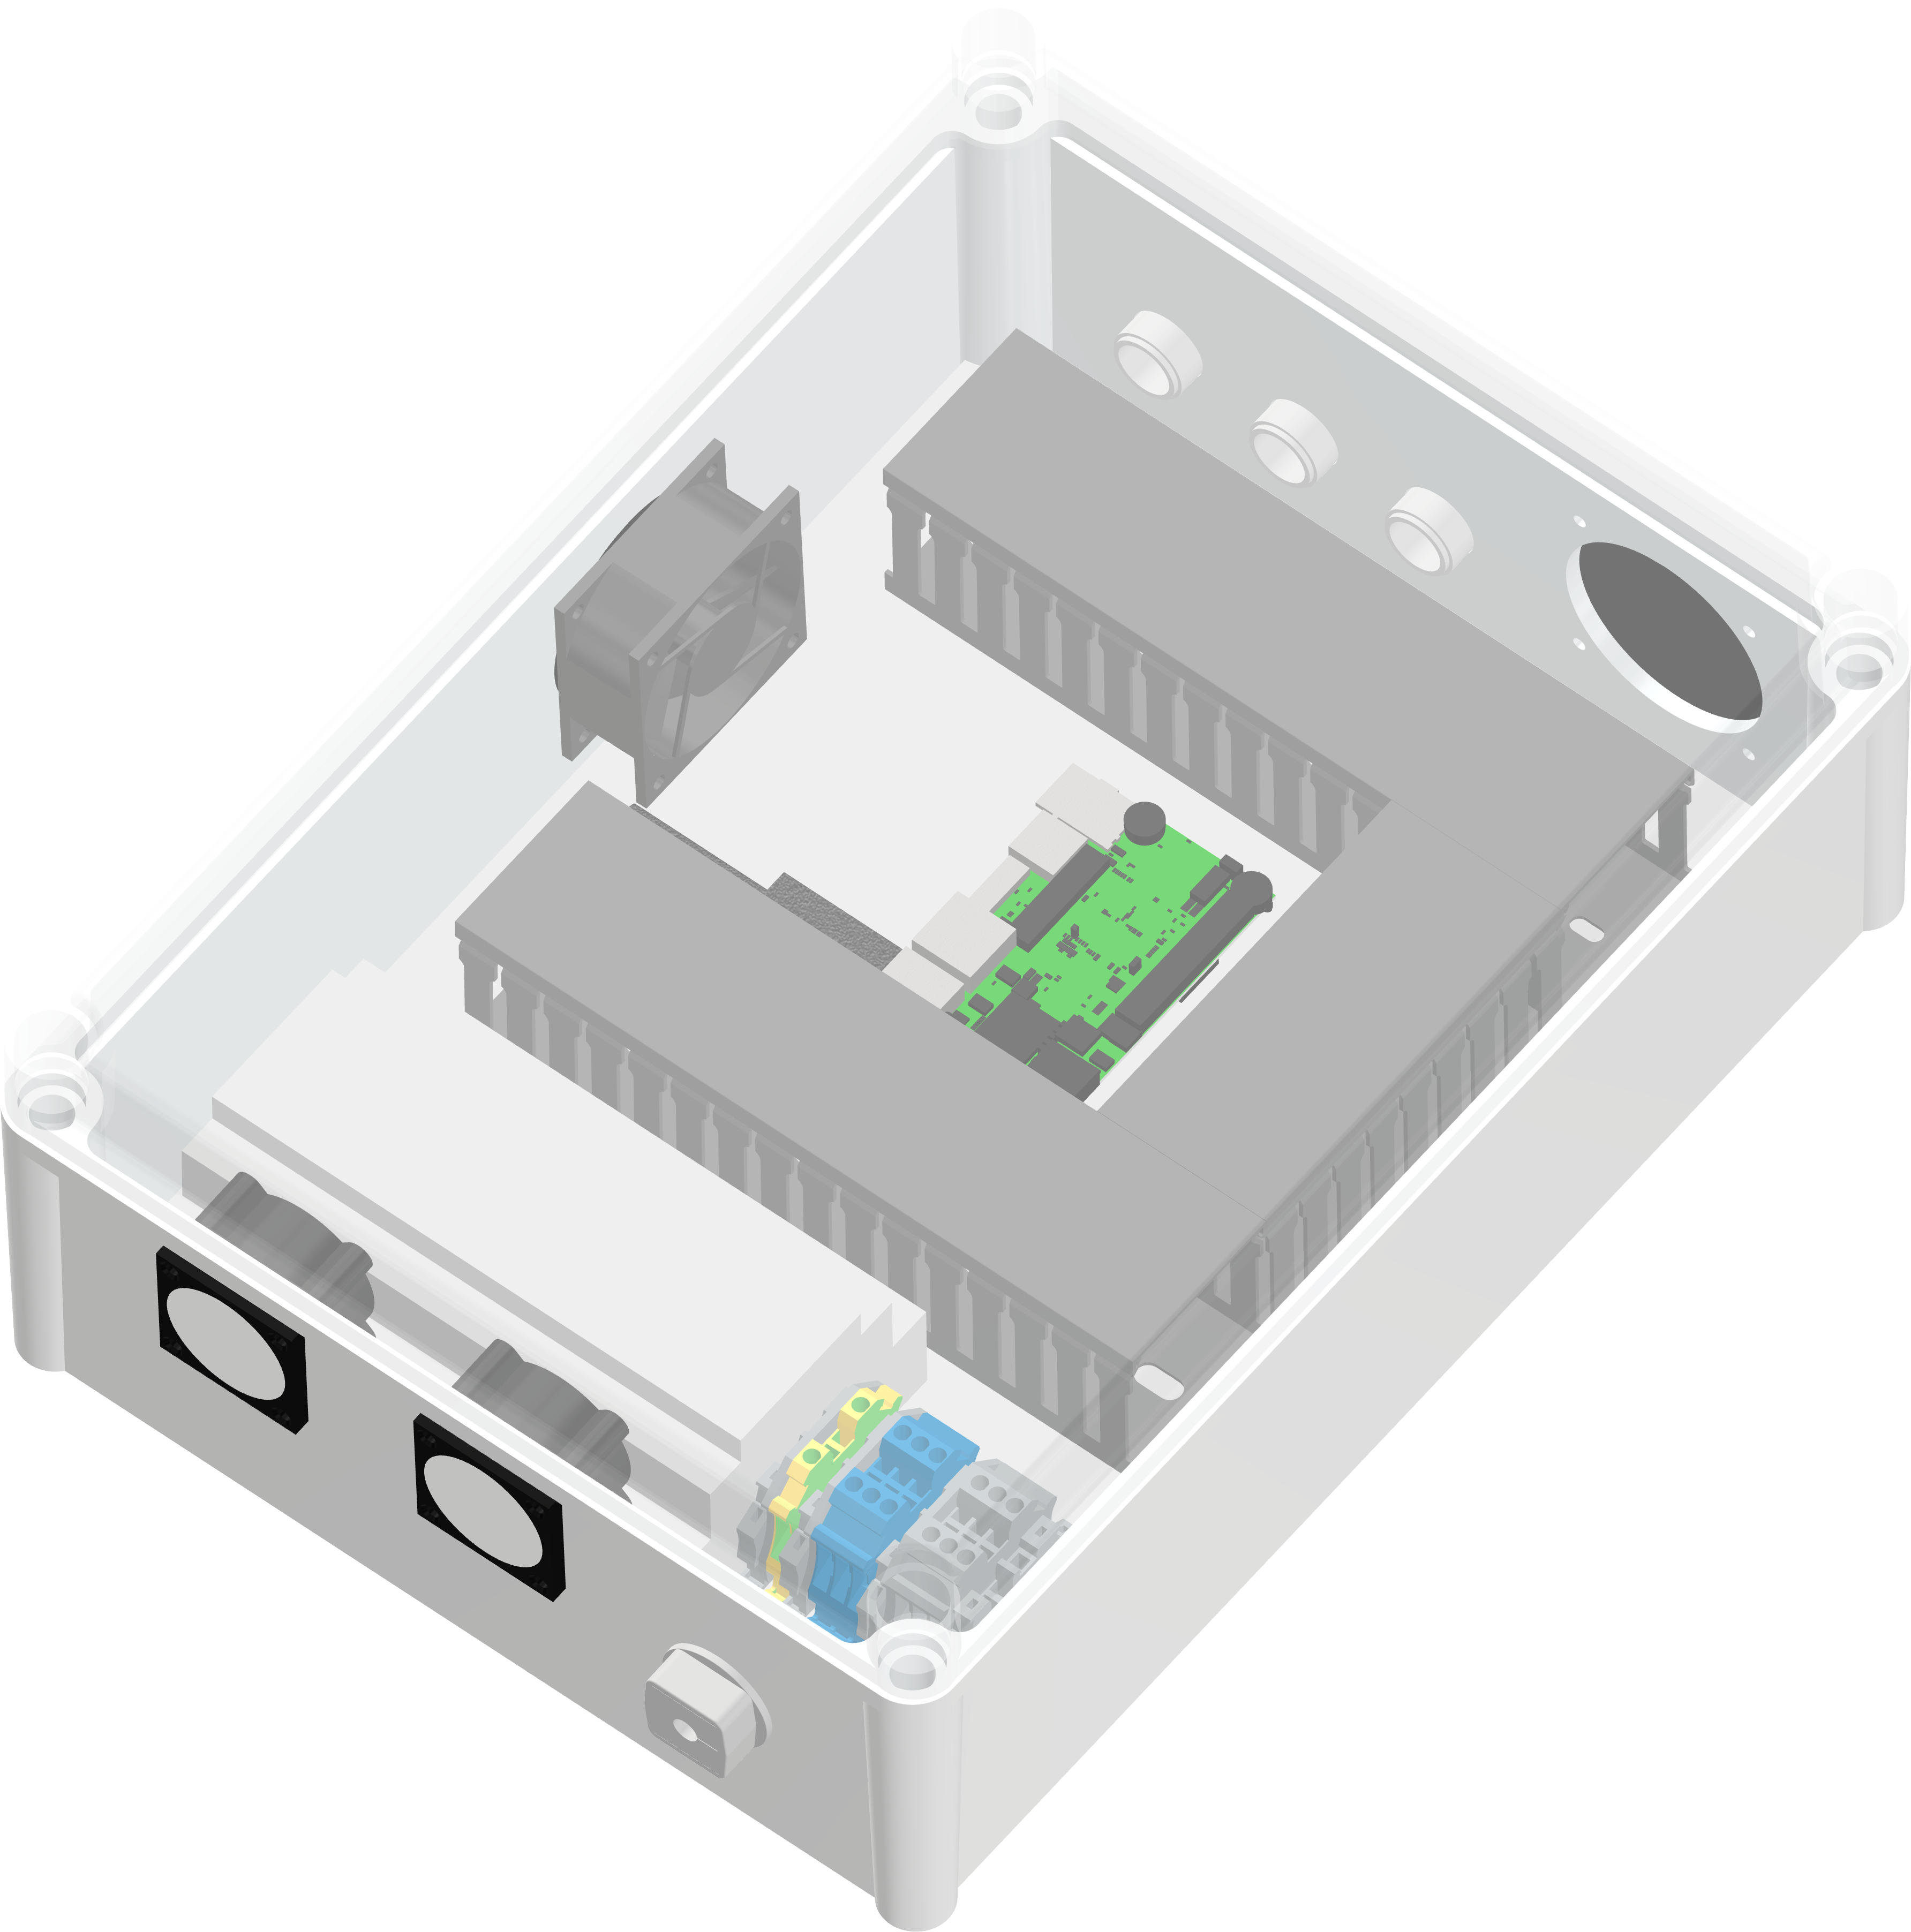
\includegraphics[width=0.5\textwidth]{graphics/case.png}
  \caption{3D model of the Fibox case}
  \label{fig:fibox3d}
\end{figure}
